\documentclass[11pt, oneside]{article} 
\usepackage{geometry}
\geometry{letterpaper} 
\usepackage{graphicx}
	
\usepackage{amssymb}
\usepackage{amsmath}
\usepackage{parskip}
\usepackage{color}
\usepackage{hyperref}

\graphicspath{{/Users/telliott/Dropbox/Github-Math/quickgeo/figures/}{/Users/telliott/Dropbox/Github-Math/figures/}}
% \begin{center} \includegraphics [scale=0.4] {gauss3.png} \end{center}

\title{Congruent triangles}
\date{}

\begin{document}
\maketitle
\Large

%[my-super-duper-separator]

A frequent task in geometry is to decide whether two shapes are congruent.  Congruence is a fancy word for equal, or the same.

There is a special symbol, a modified equals sign, for congruence ($\cong$).  For example:  
\[ \triangle ABC \cong \triangle DEF  \]

Every triangle (symbol:  $\triangle$) is constructed from three line segments, called its \emph{sides}.  Hence, each triangle has three points where its sides meet, called vertices (singular, vertex), and an angle is formed there.

\begin{center} 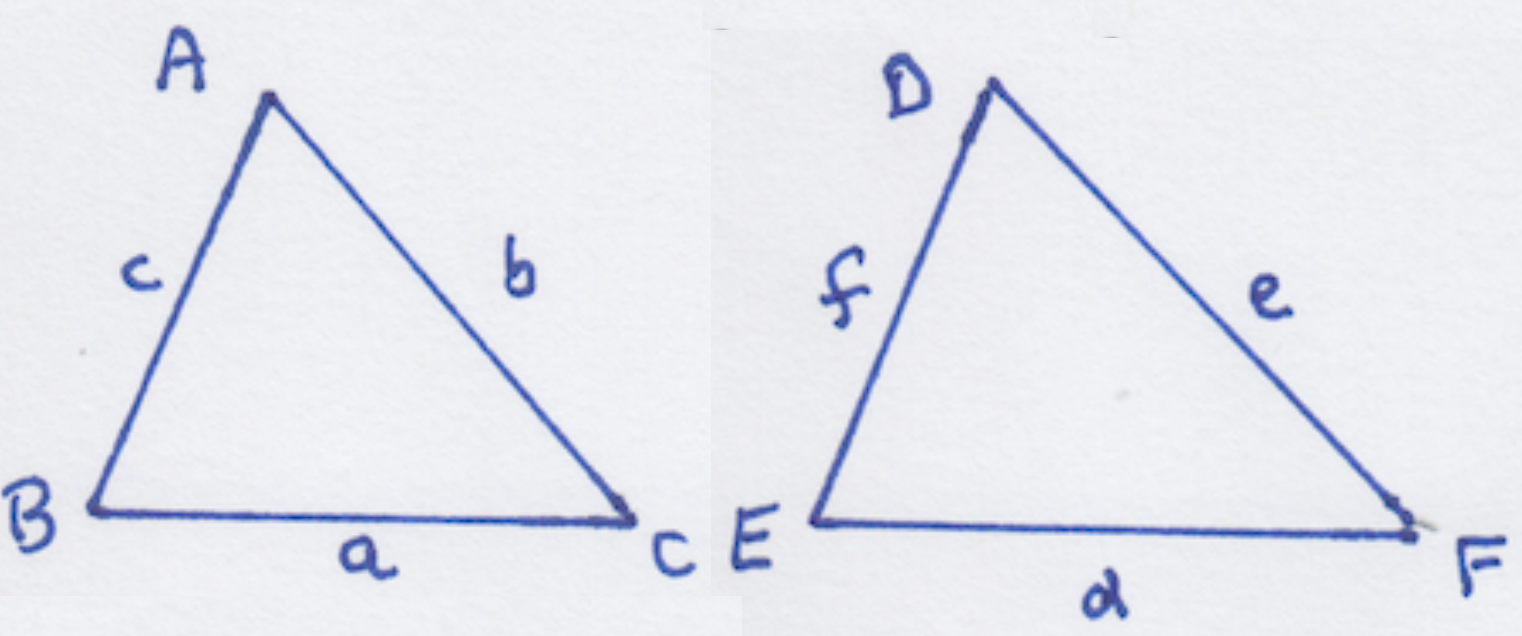
\includegraphics [scale=0.35] {C1c.png} \end{center}

When two triangles are congruent, all 3 angles and all 3 sides are equal.  $\angle A = \angle D$ and so on.  Side $a$ equals side $d$, and so on, as well.  

Also, for congruence, equal sides must lie between the corresponding angles.  But, this doesn't come up often, for the simple reason that keeping the angles the same but switching two sides usually means we don't have a triangle any more.

There is another type of relationship that we also care about, called similarity.  Two triangles are similar if they have all the angles equal.  The shape is the same but all the sides are scaled by some factor.
\begin{center} 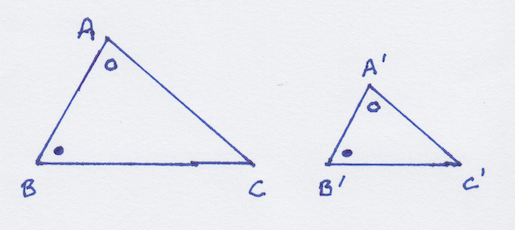
\includegraphics [scale=0.5] {C16.png} \end{center}

Because of the triangle sum theorem, we know that if any two angles are equal, then the third angle is equal as well.  Similarity is an amazingly powerful concept and we'll have a lot to say about it later.

\subsection*{rectangles}

A rectangle is defined as a four-sided figure (called a quadrilateral) with both pairs of opposite sides equal, and right angles at all four corners (only two are marked here).  Bars mark the equal sides and dots or right angle symbols mark angles that are equal.  
\begin{center} 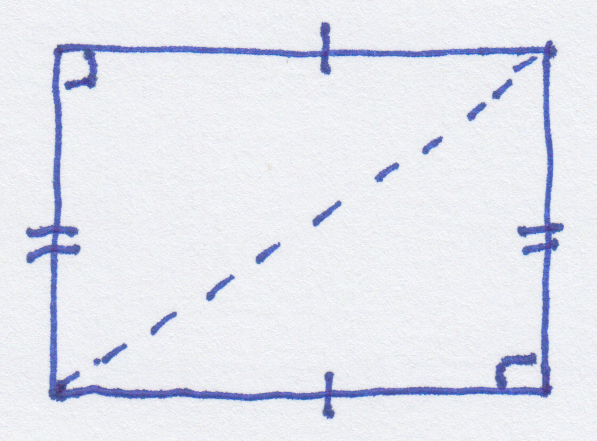
\includegraphics [scale=0.25] {C2.png} \end{center}

Think for a second what it would take to prove that two rectangles are congruent.  Clearly, you do not need all those conditions to be met.  Four right angles will do it.  One pair of equal and opposite sides and any two right angles might be enough.  How about two pairs of equal and opposite sides and one right angle?

\subsection*{Proving triangle congruence}

In the figure above the diagonal splits the rectangle into two right triangles.  Since we started with a rectangle, all four angles are right angles and the sides are equal as marked.

Our first test or method for proving congruence of triangles is called SAS, which stands for side-angle-side.  Look again at the diagonal inside the rectangle.  The long sides marked with a single cross-bar are equal, as are the other two sides.  The angle between them is also equal.  

We say that we \emph{have} (i.e. we have shown or proved) SAS, and conclude that the two triangles are congruent.  
\begin{center} 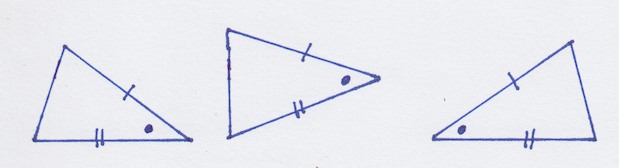
\includegraphics [scale=0.5] {C1a.png} \end{center}

In the figure above, there are three triangles each with two sides marked as equal with bars, and the angle between them marked as equal with a filled blue dot.  These triangles are all congruent, by SAS.  

Notice that one on the right is a mirror image of the others, it has undergone a \emph{reflection}.  We consider two triangles that are mirror images to be congruent.  Rotation, translation (movement from one place to another), and reflection are all allowed and two triangles can still be congruent.

\subsection*{why SAS works}

A good way to think about congruence tests is to ask how much information we need to draw a copy of an existing triangle so as to have the two be congruent.

Suppose we're starting with $\triangle ABC$
\begin{center} 
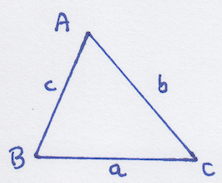
\includegraphics [scale=0.6] {C1.png} 
\end{center}

In the SAS method, think about first duplicating $\angle B$ so that $\angle B' = \angle B$.  Draw the sides as dotted lines until we know how long they should be.
\begin{center} 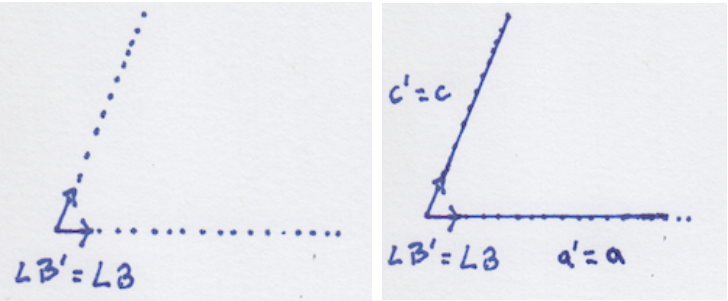
\includegraphics [scale=0.4] {C14.png} \end{center}
But that's exactly what the two side lengths gives us.  Their lengths determine the location of the other two vertices of the triangle.
\begin{center} 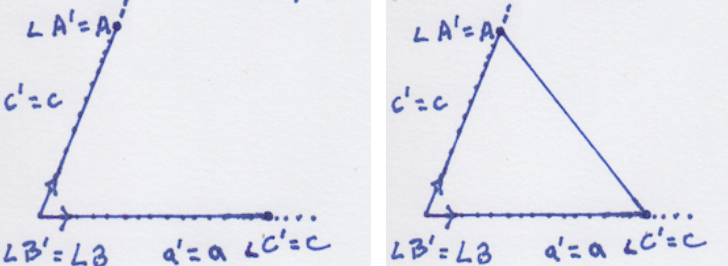
\includegraphics [scale=0.4] {C15.png} \end{center}

If you think about it you will see that switching the sides will also work.  If we draw a length $a' = a$ on the side going up, and a length $c' =c$ on the horizontal, then we will still have SAS.

The resulting triangles are mirror images of each other.  Such triangles, all 3 angles equal and all 3 sides equal, but flipped, are still congruent.

\subsection*{ASA}

A second method for establishing congruence is called angle-side-angle.
\begin{center} 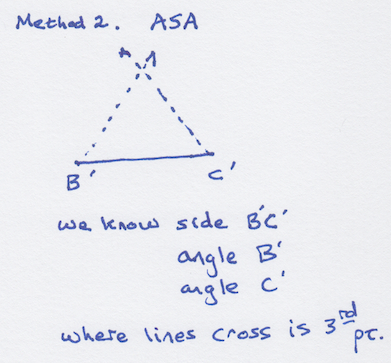
\includegraphics [scale=0.6] {C6.png} \end{center}

The diagram above shows why ASA works to determine congruent $\triangle$.

\subsection*{SSS $\rightarrow$ SAS}

A third method for proving congruence is SSS.  It is logically equivalent to SAS, but to prove this we need the isosceles triangles theorem from the next chapter.

\subsection*{right triangles}

If two triangles are both right triangles, then if any two pairs of sides are equal, the two triangles are congruent.  If both are base sides, this follows from SAS.  

If one side is the hypotenuse, what is often called HL (hypotenuse-leg), then one can swing the hypotenuse against the other base to see why it works.  Or just look forward to the Pythagorean theorem and say that if we know two sides in a right triangle, we know the third.  So again we will have SAS.


\end{document}
